\section{Presentation and Overview}

\begin{tkzexample}[latex=5cm,small]
  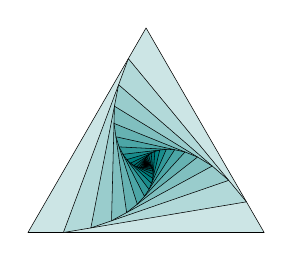
\begin{tikzpicture}[scale=.25]
  \tkzDefPoints{0/0/A,12/0/B,6/12*sind(60)/C}
  \foreach \density in {20,30,...,240}{%
    \tkzDrawPolygon[fill=teal!\density](A,B,C)
    \pgfnodealias{X}{A}
    \tkzDefPointWith[linear,K=.15](A,B) \tkzGetPoint{A}
    \tkzDefPointWith[linear,K=.15](B,C) \tkzGetPoint{B}
    \tkzDefPointWith[linear,K=.15](C,X) \tkzGetPoint{C}}
  \end{tikzpicture}
\end{tkzexample}

\vspace*{12pt}

\subsection{Why \tkzname{\tkznameofpack}? }
My initial goal was to provide other mathematics teachers and myself with a tool to quickly create Euclidean geometry figures without investing too much effort in learning a new programming language.
Of course, \tkzname{\tkznameofpack}  is for math teachers who use \LATEX\ and  makes it possible to easily create correct  drawings by means of \LATEX.

It appeared that the simplest method was to reproduce the one used to obtain construction by hand. 
To describe a construction, you must, of course, define the objects but also the actions that you perform. It seemed to me that syntax close to the language of mathematicians and their students would be more easily understandable; moreover, it also seemed to me that this syntax should be close to that of \LaTeX. 
The objects, of course, are points, segments, lines, triangles, polygons and circles. As for actions, I considered five to be sufficient, namely: define, create, draw, mark and label.

The syntax is perhaps too verbose but it is, I believe, easily accessible.
As a result, the students like teachers were able to easily access this tool.

\subsection{ \tkzname{\TIKZ } vs \tkzname{\tkznameofpack} }

I love programming with  \TIKZ,  and without  \TIKZ\  I would never have had the idea to create \tkzname{\tkznameofpack}  but never forget that behind it there is  \TIKZ\  and that it is always possible to insert code from  \TIKZ. \tkzname{\tkznameofpack}  doesn't prevent you from using  \TIKZ.
That said, I don't think mixing syntax is a good thing. 

There is no need to compare \TIKZ\  and \tkzname{\tkznameofpack}.  The latter is not addressed to the same audience as  \TIKZ. The first one allows you to do a lot of things, the second one only does geometry drawings. The first one can do everything the second one does, but the second one will more easily do what you want.

The main purpose is to define points to create geometrical figures. \tkzname{\tkznameofpack} allows you to draw the essential objects of Euclidean geometry from these points but it may be insufficient for some actions like coloring surfaces. In this case you will have to use \TIKZ\   which is always possible.

Here are some comparisons between \tkzname{\TIKZ } and \tkzname{\tkznameofpack} 4. For this I will use the geometry examples from the PGFManual.
  The two most important Euclidean tools used by early Greeks to construct different geometrical shapes and angles were a compass and a straightedge. My idea is to allow you to follow step by step a construction that would be done by hand (with compass and straightedge) as naturally as possible.

\subsubsection{Book I, proposition I  \_Euclid's Elements\_ }

\begin{tikzpicture}
\node [mybox,title={Book I, proposition I  \_Euclid's Elements\_}] (box){%
    \begin{minipage}{0.90\textwidth}
{\emph{To construct an equilateral triangle on a given finite straight line.}
} 
    \end{minipage}
};
\end{tikzpicture}% 


Explanation :

The fourth tutorial of the \emph{PgfManual} is about geometric constructions. \emph{T. Tantau} proposes to get the drawing with its beautiful tool Ti\emph{k}Z. Here I propose the same construction with \emph{tkz-elements}. The color of the Ti\emph{k}Z code is orange and that of \emph{tkz-elements} is red.

\medskip

\hspace*{1cm}\vbox{\color{orange} |\usepackage{tikz}|\\
|\usetikzlibrary{calc,intersections,through,backgrounds}|}

\medskip
\hspace*{1cm}\vbox{\color{red} |\usepackage{tkz-euclide}|}

\medskip
How to get the line AB ? To get this line, we use two fixed points.\\

\medskip
\hspace*{1cm}\vbox{\color{orange} 
|\coordinate [label=left:$A$] (A) at (0,0);|\\
|\coordinate [label=right:$B$] (B) at (1.25,0.25);|\\
|\draw (A) -- (B);|}

\medskip
\hspace*{1cm}\vbox{\color{red}
|\tkzDefPoint(0,0){A}|\\
|\tkzDefPoint(1.25,0.25){B}|\\
|\tkzDrawSegment(A,B)|\\
|\tkzLabelPoint[left](A){$A$}|\\
|\tkzLabelPoint[right](B){$B$}|}

We want to draw a circle around the points $A$ and $B$ whose radius is given by the length of the line AB. 
\medskip

\hspace*{1cm}\vbox{\color{orange}
|\draw let \p1 = ($ (B) - (A) $),|\\
|\n2 = {veclen(\x1,\y1)} in|\\
|          (A) circle (\n2)|\\
|          (B) circle (\n2);|}

\medskip
\hspace*{1cm}\vbox{\color{red} 
|\tkzDrawCircles(A,B B,A)|
}

The intersection of the circles $\mathcal{D}$ and $\mathcal{E}$

\medskip

\hspace*{1cm}\vbox{\color{orange} 
|draw [name path=A--B] (A) -- (B);|\\
|node (D) [name path=D,draw,circle through=(B),label=left:$D$] at (A) {}; |\\
|node (E) [name path=E,draw,circle through=(A),label=right:$E$] at (B) {};|\\
|path [name intersections={of=D and E, by={[label=above:$C$]C, [label=below:$C'$]C'}}]; |\\
|draw [name path=C--C',red] (C) -- (C');|\\
|path [name intersections={of=A--B and C--C',by=F}];|\\
|node [fill=red,inner sep=1pt,label=-45:$F$] at (F) {};|\\}

\medskip
\hspace*{1cm}\vbox{\color{red} |\tkzInterCC(A,B)(B,A) \tkzGetPoints{C}{X}|\\}


How to draw points :

\medskip
\hspace*{1cm}\vbox{\color{orange} |\foreach \point in {A,B,C}|\\
|\fill [black,opacity=.5] (\point) circle (2pt);|\\}

\medskip
\hspace*{1cm}\vbox{\color{red}| \tkzDrawPoints[fill=gray,opacity=.5](A,B,C)|\\}

\subsubsection{Complete code with \pkg{tkz-euclide}}

We need to define colors 

|\colorlet{input}{red!80!black} |\\
|\colorlet{output}{red!70!black}|\\
|\colorlet{triangle}{orange!40}  |

\begin{tkzexample}[vbox,small]
  \colorlet{input}{red!80!black} 
  \colorlet{output}{red!70!black}
  \colorlet{triangle}{orange!40}
  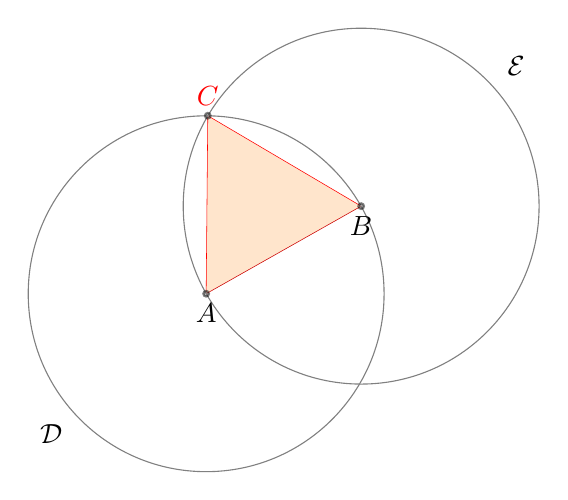
\begin{tikzpicture}[scale=1.25,thick,help lines/.style={thin,draw=black!50}]
  \tkzDefPoint(0,0){A}     
  \tkzDefPoint(1.25+rand(),0.25+rand()){B}      
  \tkzInterCC(A,B)(B,A) \tkzGetPoints{C}{X}

  \tkzFillPolygon[triangle,opacity=.5](A,B,C)
  \tkzDrawSegment[input](A,B) 
  \tkzDrawSegments[red](A,C B,C)  
  \tkzDrawCircles[help lines](A,B B,A)
  \tkzDrawPoints[fill=gray,opacity=.5](A,B,C)
  
  \tkzLabelPoints(A,B)
  \tkzLabelCircle[below=12pt](A,B)(180){$\mathcal{D}$}
  \tkzLabelCircle[above=12pt](B,A)(180){$\mathcal{E}$}
  \tkzLabelPoint[above,red](C){$C$}
      
  \end{tikzpicture}
\end{tkzexample}

\subsubsection{Book I, Proposition II  \_Euclid's Elements\_}

\begin{tikzpicture}
\node [mybox,title={Book I, Proposition II  \_Euclid's Elements\_}] (box){%
\begin{minipage}{0.90\textwidth}
  {\emph{To place a straight line equal to a given straight line with one end at a given point.}} 
\end{minipage}
};
\end{tikzpicture}% 

Explanation

In the first part, we need to find the midpoint of the straight line $AB$. With \TIKZ\ we can use the calc library

\medskip
\hspace*{1cm}\vbox{\color{orange} |\coordinate [label=left:$A$] (A) at (0,0);|\\
|\coordinate [label=right:$B$] (B) at (1.25,0.25);|\\
|\draw (A) -- (B);|\\
|\node [fill=red,inner sep=1pt,label=below:$X$] (X) at ($ (A)!.5!(B) $) {};|\\}

With \pkg{tkz-euclide} we have a macro \tkzcname{tkzDefMidPoint}, we get the point X with \tkzcname{tkzGetPoint} but we don't need this point to get the next step.


\medskip
\hspace*{1cm}\vbox{\red |\tkzDefPoints{0/0/A,0.75/0.25/B,1/1.5/C}|\\  
|\tkzDefMidPoint(A,B) \tkzGetPoint{X}|}\\

\medskip
Then we need to construct a triangle equilateral. It's easy with \pkg{tkz-euclide} . With TikZ you need some effort because you need to use the midpoint $X$ to get the point $D$ with trigonometry calculation.

\medskip
\hspace*{1cm}\vbox{\color{orange}
|\node [fill=red,inner sep=1pt,label=below:$X$] (X) at ($ (A)!.5!(B) $) {}; | \\
|\node [fill=red,inner sep=1pt,label=above:$D$] (D) at                      |  \\
|($ (X) ! {sin(60)*2} ! 90:(B) $) {};                                       |  \\
|\draw (A) -- (D) -- (B);                                                   |  \\
}                                                                           \\

\medskip
\hspace*{1cm}\vbox{\color{red} |\tkzDefTriangle[equilateral](A,B) \tkzGetPoint{D}|}\\

We can draw the triangle at the end of the picture with

\medskip
\hspace*{1cm}\vbox{\color{red} |\tkzDrawPolygon{A,B,C}|}

\medskip
We know how to draw the circle  $\mathcal{H}$ around $B$ through $C$ and how to place the points $E$ and $F$

\medskip
\hspace*{1cm}\vbox{\color{orange} 
|\node (H) [label=135:$H$,draw,circle through=(C)] at (B) {};|          \\
|\draw (D) -- ($ (D) ! 3.5 ! (B) $) coordinate [label=below:$F$] (F);|  \\
|\draw (D) -- ($ (D) ! 2.5 ! (A) $) coordinate [label=below:$E$] (E);|} \\

\medskip

\hspace*{1cm}\vbox{\color{red} |\tkzDrawCircle(B,C)|\\
|\tkzDrawLines[add=0 and 2](D,A D,B)|}

\medskip
We can place the points $E$ and $F$ at the end of the picture. We don't need them now.

Intersecting a Line and a Circle : here we search the intersection of the circle around $B$ through $C$ and the line $DB$.
The infinite straight line $DB$ intercepts the circle but with \TIKZ\ we need to extend the lines  $DB$  and that can be done using partway calculations. We get the point $F$ and $BF$ or $DF$ intercepts the circle

\medskip
\hspace*{1cm}\vbox{\color{orange}| \node (H) [label=135:$H$,draw,circle through=(C)] at (B) {}; |  \\
|\path let \p1 = ($ (B) - (C) $) in|                                     \\
|  coordinate [label=left:$G$] (G) at ($ (B) ! veclen(\x1,\y1) ! (F) $); |  \\
|\fill[red,opacity=.5] (G) circle (2pt);|}                                \\

\medskip
Like the intersection of two circles, it's easy to find the intersection of a line and a circle with \pkg{tkz-euclide}. We don't need $F$ 

\medskip
\hspace*{1cm}\vbox{\color{red} | \tkzInterLC(B,D)(B,C)\tkzGetFirstPoint{G}|}

\medskip
There are no more difficulties. Here the final code with some simplications.
We draw the circle $\mathcal{K}$ with center $D$ and passing through $G$. It intersects the line $AD$ at point $L$. $AL = BC$.

\hspace*{1cm}\vbox{\color{red} | \tkzDrawCircle(D,G)|}
\hspace*{1cm}\vbox{\color{red} | \tkzInterLC(D,A)(D,G)\tkzGetSecondPoint{L}|}

\begin{tkzexample}[latex=7cm,small]
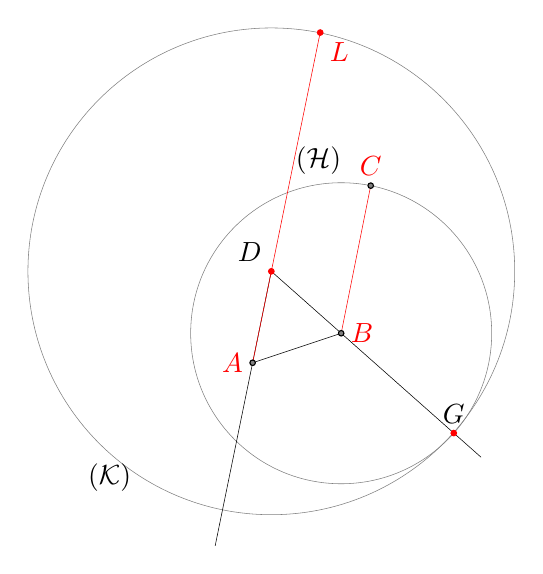
\begin{tikzpicture}[scale=1.5]
\tkzDefPoint(0,0){A}
\tkzDefPoint(0.75,0.25){B}  
\tkzDefPoint(1,1.5){C} 
\tkzDefTriangle[equilateral](A,B)   \tkzGetPoint{D}
\tkzInterLC[near](D,B)(B,C)    \tkzGetSecondPoint{G}
\tkzInterLC[near](D,A)(D,G)    \tkzGetFirstPoint{L}
\tkzDrawCircles(B,C D,G)
\tkzDrawLines[add=0 and 2](D,A D,B)
\tkzDrawSegment(A,B) 
\tkzDrawSegments[red](A,L B,C) 
\tkzDrawPoints[red](D,L,G)
\tkzDrawPoints[fill=gray](A,B,C)
\tkzLabelPoints[left,red](A)
\tkzLabelPoints[below right,red](L)
\tkzLabelCircle[above](B,C)(20){$\mathcal{(H)}$}
\tkzLabelPoints[above left](D)
\tkzLabelPoints[above](G)
\tkzLabelPoints[above,red](C)
\tkzLabelPoints[right,red](B)
\tkzLabelCircle[below](D,G)(-90){$\mathcal{(K)}$}
\end{tikzpicture}
\end{tkzexample}

\subsection{\tkzname{\tkznameofpack 4}   vs \tkzname{\tkznameofpack 3}}

Now I am no longer a Mathematics teacher, and I only spend a few hours studying geometry. I wanted to avoid multiple complications by trying to make \tkzname{tkz-euclide} independent of \tkzname{tkz-base}. Thus was born \tkzname{\tkznameofpack} 4. The latter is a simplified version of its predecessor. The macros of \tkzname{tkz-euclide 3} have been retained. The unit is now  \tkzname{cm}.  If you need some macros from \tkzname{tkz-base}, you may need to use the \tkzcname{tkzInit}.

\subsection{How to use the \tkzname{\tkznameofpack} package ?}
\subsubsection{Let's look at a classic example}
In order to show the right way, we will see how to build an equilateral triangle. Several possibilities are open to us, we are going to follow the steps of Euclid.

\begin{itemize}
\item   First of all, you have to use a document class. The best choice to test your code is to create a single figure with the class \tkzname{standalone}\index{standalone}.
\begin{verbatim}  
\documentclass{standalone}
\end{verbatim}
\item Then load the \tkzname{\tkznameofpack} package:
\begin{verbatim}  
\usepackage{tkz-euclide}
\end{verbatim}

 You don't need to load \TIKZ\ because the \tkzname{\tkznameofpack} package works on top of TikZ and loads it.

 \item Start the document and open a TikZ picture environment:
\begin{verbatim}
\begin{document}
\begin{tikzpicture}
\end{verbatim}

\item Now we define two fixed points:
\begin{verbatim}
\tkzDefPoint(0,0){A}
\tkzDefPoint(5,2){B}
\end{verbatim}

\item Two points define two circles, let's use these circles:

 circle with center $A$ through $B$ and circle with center $B$ through $A$. These two circles have two points in common.
\begin{verbatim}
\tkzInterCC(A,B)(B,A)
\end{verbatim}
We can get the points of intersection with
\begin{verbatim}
\tkzGetPoints{C}{D}
\end{verbatim}

\item All the necessary points are obtained, we can move on to the final steps including the plots.
\begin{verbatim}
\tkzDrawCircles[gray,dashed](A,B B,A)
\tkzDrawPolygon(A,B,C)% The triangle
\end{verbatim}
\item Draw all points $A$, $B$, $C$ and $D$:
\begin{verbatim}
\tkzDrawPoints(A,...,D)
\end{verbatim}

\item The final step, we print labels to the points and use options for positioning:\\
\begin{verbatim}
\tkzLabelSegments[swap](A,B){$c$}
\tkzLabelPoints(A,B,D)
\tkzLabelPoints[above](C)
\end{verbatim}
\item We finally close both environments
\begin{verbatim}
\end{tikzpicture}
\end{document}
\end{verbatim}

\item The complete code

\begin{tkzexample}[latex=8cm,small]
 \begin{tikzpicture}[scale=.5]
   % fixed points
  \tkzDefPoint(0,0){A}
  \tkzDefPoint(5,2){B}
  % calculus
  \tkzInterCC(A,B)(B,A)
  \tkzGetPoints{C}{D}
  % drawings
  \tkzDrawCircles(A,B B,A)
  \tkzDrawPolygon(A,B,C)
  \tkzDrawPoints(A,...,D)
  % marking
  \tkzMarkSegments[mark=s||](A,B B,C C,A)
  % labelling
  \tkzLabelSegments[swap](A,B){$c$}
  \tkzLabelPoints(A,B,D)
  \tkzLabelPoints[above](C)
\end{tikzpicture}
\end{tkzexample}

 \end{itemize}

\subsubsection{ Part I: golden triangle}
\begin{center}
\begin{tikzpicture}
  
\tkzDefPoint(0,0){C} % possible \tkzDefPoint[label=below:$C$](0,0){C} but don't do this
\tkzDefPoint(2,6){B}
% We get D and E with a rotation
\tkzDefPointBy[rotation= center B angle 36](C) \tkzGetPoint{D} 
\tkzDefPointBy[rotation= center B angle 72](C) \tkzGetPoint{E} 
% Toget A we use an intersection of lines
\tkzInterLL(B,E)(C,D) \tkzGetPoint{A}
\tkzInterLL(C,E)(B,D) \tkzGetPoint{H}

% angles 
\tkzMarkAngles[size=2](C,B,D E,A,D) %this is to draw the arcs
\tkzLabelAngles[pos=1.5](C,B,D E,A,D){$\alpha$}
\tkzMarkRightAngle(B,H,C)
\tkzDrawPoints(A,...,E)

% drawing
\tkzDrawArc[delta=10](B,C)(E)
\tkzDrawPolygon(C,B,D)
\tkzDrawSegments(D,A B,A C,E)

% Label only now
\tkzLabelPoints[below left](C,A)
\tkzLabelPoints[below right](D)
\tkzLabelPoints[above](B,E)
\end{tikzpicture}
\end{center}

Let's analyze the figure
\begin{enumerate}
  \item $CBD$ and $DBE$ are isosceles triangles; 
  
  \item $BC=BE$ and $(BD)$ is a bisector of the angle $CBE$;
  
  \item From this we deduce that the $CBD$ and $DBE$ angles are equal and have the same measure $\alpha$
   \[\widehat{BAC} +\widehat{ABC} + \widehat{BCA}=180^\circ \ \text{in the triangle}\ BAC \]
   \[3\alpha + \widehat{BCA}=180^\circ\  \text{in the triangle}\ CBD\]
   then 
     \[\alpha + 2\widehat{BCA}=180^\circ \] 
   or 
     \[\widehat{BCA}=90^\circ -\alpha/2 \] 
    
    \item  Finally   \[\widehat{CBD}=\alpha=36^\circ \] 
     the triangle $CBD$ is a "golden" triangle.
\end{enumerate}

\vspace*{24pt}
How construct a golden triangle or an angle of $36^\circ$?

\begin{enumerate}
  \item We place the fixed points $C$ and $D$. |\tkzDefPoint(0,0){C}| and |\tkzDefPoint(4,0){D}|;
  \item  We construct a square $CDef$ and we construct the midpoint $m$ of $[Cf]$;
  
  We can do all of this with a compass and a rule;
  \item Then we trace an arc with center $m$ through $e$. This arc cross the line $(Cf)$ at $n$;
  \item Now the two arcs with center $C$ and $D$ and radius $Cn$ define the point $B$.
\end{enumerate}

\begin{tkzexample}[latex=7cm,small]
\begin{tikzpicture}
  \tkzDefPoint(0,0){C}
  \tkzDefPoint(4,0){D}
  \tkzDefSquare(C,D)                     
  \tkzGetPoints{e}{f}
  \tkzDefMidPoint(C,f)                   
  \tkzGetPoint{m}
  \tkzInterLC(C,f)(m,e)                  
  \tkzGetSecondPoint{n}
  \tkzInterCC[with nodes](C,C,n)(D,C,n) 
  \tkzGetFirstPoint{B}
  \tkzDrawSegment[brown,dashed](f,n)
  \pgfinterruptboundingbox% from tikz
  \tkzDrawPolygon[brown,dashed](C,D,e,f)
  \tkzDrawArc[brown,dashed](m,e)(n)
  \tkzCompass[brown,dashed,delta=20](C,B)
  \tkzCompass[brown,dashed,delta=20](D,B)
  \endpgfinterruptboundingbox 
  \tkzDrawPolygon(B,...,D)
  \tkzDrawPoints(B,C,D,e,f,m,n)
  \tkzLabelPoints[above](B)
  \tkzLabelPoints[left](f,m,n)
  \tkzLabelPoints(C,D)
  \tkzLabelPoints[right](e)
\end{tikzpicture}
\end{tkzexample}


After building the golden triangle $BCD$, we build the point $A$ by noticing that $BD=DA$. Then we get the point $E$ and finally the point $F$. This is done with already intersections of defined objects  (line and circle).


\subsubsection{Part II: two others methods with golden and euclid triangle}

\tkzname{\tkznameofpack} knows how to define a "golden" or "euclide" triangle. We can define $BCD$ and $BCA$ like gold triangles.


  \begin{center}
    \begin{tkzexample}[code only,small]
      \begin{tikzpicture}
        \tkzDefPoint(0,0){C}
        \tkzDefPoint(4,0){D}
        \tkzDefTriangle[golden](C,D)
        \tkzGetPoint{B}
        \tkzDefTriangle[golden](B,C)
        \tkzGetPoint{A}
        \tkzInterLC(B,A)(B,D) \tkzGetSecondPoint{E}
        \tkzInterLL(B,D)(C,E) \tkzGetPoint{F}
        \tkzDrawPoints(C,D,B)
        \tkzDrawPolygon(B,...,D)  
        \tkzDrawPolygon(B,C,D)
        \tkzDrawSegments(D,A A,B C,E)
        \tkzDrawArc[delta=10](B,C)(E)
        \tkzDrawPoints(A,...,F) 
        \tkzMarkRightAngle(B,F,C)  
        \tkzMarkAngles(C,B,D E,A,D)
        \tkzLabelAngles[pos=1.5](C,B,D E,A,D){$\alpha$} 
        \tkzLabelPoints[below](A,C,D,E)
        \tkzLabelPoints[above right](B,F)
      \end{tikzpicture} 
    \end{tkzexample}
  \end{center}

Here is a final method that uses rotations:  

\begin{center}
  \begin{tkzexample}[code only,small]
  \begin{tikzpicture} 
  \tkzDefPoint(0,0){C} % possible 
  % \tkzDefPoint[label=below:$C$](0,0){C} 
  % but don't do this
  \tkzDefPoint(2,6){B}
  % We get D and E with a rotation
  \tkzDefPointBy[rotation= center B angle 36](C) \tkzGetPoint{D} 
  \tkzDefPointBy[rotation= center B angle 72](C) \tkzGetPoint{E} 
  % To get A we use an intersection of lines
  \tkzInterLL(B,E)(C,D) \tkzGetPoint{A}
  \tkzInterLL(C,E)(B,D) \tkzGetPoint{H}
  % drawing
  \tkzDrawArc[delta=10](B,C)(E)
  \tkzDrawPolygon(C,B,D)
  \tkzDrawSegments(D,A B,A C,E)
  % angles 
  \tkzMarkAngles(C,B,D E,A,D) %this is to draw the arcs
  \tkzLabelAngles[pos=1.5](C,B,D E,A,D){$\alpha$}
  \tkzMarkRightAngle(B,H,C)
  \tkzDrawPoints(A,...,E)
  % Label only now
  \tkzLabelPoints[below left](C,A)
  \tkzLabelPoints[below right](D)
  \tkzLabelPoints[above](B,E)
  \end{tikzpicture}
  \end{tkzexample}
\end{center}


\subsubsection{Complete but minimal example}


A unit of length being chosen, the example shows how to obtain a segment of length $\sqrt{a}$ from a segment of length $a$, using a ruler and a compass.

$IB=a$, $AI=1$

\vspace{12pt}
\hypertarget{firstex}{}
\begin{tkzexample}[vbox,small]
\begin{tikzpicture}[scale=1,ra/.style={fill=gray!20}]
   % fixed points
   \tkzDefPoint(0,0){A}
   \tkzDefPoint(1,0){I}
   % calculation
   \tkzDefPointBy[homothety=center A ratio  10 ](I) \tkzGetPoint{B}  
   \tkzDefMidPoint(A,B)              \tkzGetPoint{M}
   \tkzDefPointWith[orthogonal](I,M) \tkzGetPoint{H}
   \tkzInterLC(I,H)(M,B)             \tkzGetFirstPoint{C}
   \tkzDrawSegment[style=orange](I,C)
   \tkzDrawArc(M,B)(A)
   \tkzDrawSegment[dim={$1$,-16pt,}](A,I)
   \tkzDrawSegment[dim={$a/2$,-10pt,}](I,M)
   \tkzDrawSegment[dim={$a/2$,-16pt,}](M,B)   
   \tkzMarkRightAngle[ra](A,I,C)
   \tkzDrawPoints(I,A,B,C,M)  
   \tkzLabelPoint[left](A){$A(0,0)$} 
   \tkzLabelPoints[above right](I,M)
   \tkzLabelPoints[above left](C)
   \tkzLabelPoint[right](B){$B(10,0)$}
   \tkzLabelSegment[right=4pt](I,C){$\sqrt{a^2}=a \ (a>0)$}
\end{tikzpicture}
\end{tkzexample}

\emph{Comments}
 
\begin{itemize}
\item The Preamble


 Let us first look at the preamble. If you need it, you have to load \tkzname{xcolor} before \tkzname{tkz-euclide}, that is, before \TIKZ. \TIKZ\ may cause problems with the active characters, but...
 provides a library in its latest version that's supposed to solve these problems \NameLib{babel}.
 
\begin{tkzltxexample}[]
\documentclass{standalone} % or another class
   % \usepackage{xcolor} % before tikz or tkz-euclide if necessary
\usepackage{tkz-euclide} % no need to load TikZ
   % \usetkzobj{all}  is no longer necessary 
   % \usetikzlibrary{babel}  if there are problems with the active characters
\end{tkzltxexample}

The following code consists of several parts:

   \item  Definition of fixed points: the first part includes the definitions of the points necessary for the construction, these are the fixed points. The macros \tkzcname{tkzInit} and \tkzcname{tkzClip} in most cases are not necessary.

\begin{tkzltxexample}[]
  \tkzDefPoint(0,0){A}
  \tkzDefPoint(1,0){I}
\end{tkzltxexample}
 
  \item The second part is dedicated to the creation of new points from the fixed points;
  a $B$ point is placed at $10$~cm    from $A$. The middle of $[AB]$ is defined by $M$ and then the orthogonal line to the $(AB)$ line is searched for at the $I$ point. Then we look for the intersection of this line with the semi-circle of center $M$ passing through $A$.  
  
\begin{tkzltxexample}[]
   \tkzDefPointBy[homothety=center A ratio  10 ](I)
      \tkzGetPoint{B}
   \tkzDefMidPoint(A,B)
      \tkzGetPoint{M}
   \tkzDefPointWith[orthogonal](I,M)
      \tkzGetPoint{H}
   \tkzInterLC(I,H)(M,B)             
   \tkzGetSecondPoint{C}
 \end{tkzltxexample}  
     

 \item The third one includes the different drawings;
 \begin{tkzltxexample}[]
   \tkzDrawSegment[style=orange](I,H)
   \tkzDrawPoints(O,I,A,B,M)
   \tkzDrawArc(M,A)(O)
   \tkzDrawSegment[dim={$1$,-16pt,}](A,I)
   \tkzDrawSegment[dim={$a/2$,-10pt,}](I,M)
   \tkzDrawSegment[dim={$a/2$,-16pt,}](M,B)
 \end{tkzltxexample}
 
\item  Marking: the fourth is devoted to marking;


\begin{tkzltxexample}[]
 \tkzMarkRightAngle[ra](A,I,C)
 \end{tkzltxexample}
 
 \item Labelling: the latter only deals with the placement of labels.
\begin{tkzltxexample}[]
   \tkzLabelPoint[left](A){$A(0,0)$} 
   \tkzLabelPoint[right](B){$B(10,0)$}
   \tkzLabelSegment[right=4pt](I,C){$\sqrt{a^2}=a \ (a>0)$}
\end{tkzltxexample}

\end{itemize}

\endinput